\documentclass[numbers=noenddot, 12pt, a4paper, oneside]{scrbook}
\usepackage{blindtext}
\usepackage[utf8]{inputenc}
\usepackage{float}
\usepackage{tabularx}
\usepackage{graphicx}
\def\Plus{\texttt{+}}
\usepackage{listings}
\usepackage{color}

\definecolor{dkgreen}{rgb}{0,0.6,0}
\definecolor{gray}{rgb}{0.5,0.5,0.5}
\definecolor{mauve}{rgb}{0.58,0,0.82}

\lstset{frame=tb,
	language=Java,
	aboveskip=3mm,
	belowskip=3mm,
	showstringspaces=false,
	columns=flexible,
	basicstyle={\small\ttfamily},
	numbers=none,
	numberstyle=\tiny\color{gray},
	keywordstyle=\color{blue},
	commentstyle=\color{dkgreen},
	stringstyle=\color{mauve},
	breaklines=false,
	breakatwhitespace=true,
	tabsize=3
}


\begin{document}

\begin{titlepage}
	\centering
	{\scshape\LARGE Politecnico di Milano \par}
	\vspace{1cm}
	
\includegraphics[width=0.35\textwidth]{polimi-logo}\par
	\vspace{1cm}

	{\scshape\Large Design and Implementation of Mobile Applications\par}
	\vspace{1.5cm}
	{\huge\bfseries iSport \par}
	\vspace{1cm}
	{\Large\bfseries Design Document \par}
	\vspace{3cm}
	{\Large\itshape di\par}
	{\Large\itshape Gianluigi Oliva\par}
	\vspace{1.5cm}
	\vfill
	


	\vfill

	% Bottom of the page
	{\large \today\par}
\end{titlepage}

\newpage
\tableofcontents
\newpage


\chapter{Introduction}

\section{Purpose}
Questo documento descrive le fasi di progettazione e prototipazione per la realizzazione dell'applicazione mobile "iSport". in dettaglio, verranno discussi i componenti principali, le funzionalità e l'esperienza dell'utente.

iSport è una applicazione in cui obiettivo principale è la visualizzazione di informazioni e dati relativi al mondo dello sport. In particolare ci si focalizzerà sulle notizie giornalistiche più rilevanti e sui dati relativi alle partite di calcio della giornata.

Questo progetto è il risultato dell'implementazione delle conoscenze acquisite durante il corso "Design and Implementation of Mobile Applications" fornito dal Politecnico di Milano.

\section{Intended Audience}
This document is produced for those who develop, evaluate and use iSport mobile application:
\begin{itemize}
	\item The engineers who had the idea and developed the application.
	\item The testers that must verify the effective implementation of all the described components and functions.
	\item The user who will use the application and take advantage of its functionalities.
	\item The future contributors who wish to develop new features.
\end{itemize}

\section{Definitions, acronyms, abbreviations}
\subsection*{Definitions}
\begin{itemize}
	\item \textbf{Platform}: The application as a whole.
	\item \textbf{User}: An end user who will use the application
	\item \textbf{Match}: A match between two teams that has already occurred or is in progress
	\item \textbf{Framework}: Reusable set of libraries or classes for a software system.
	\item \textbf{News}: Una notizia relativa al mondo dello sport presente su qualche rivista giornalistica
	\item \textbf{Pronostico}: Una previsione sul risultato di un match appartenente ad una classe di previsioni possibili
	\item \textbf{Quota}: Il valore di retribuzione di un pronostico relativo ad un determinato match
	\item \textbf{REST}: is a way of providing interoperability between computer systems on the Internet.
\end{itemize}
\subsection*{Acronyms}
\begin{itemize}
	\item \textbf{MVC}: Model - View - Controller
	\item \textbf{HTTPS}: HyperText Transfer Protocol Secure
	\item \textbf{IDE}: Integrated Development Environment
	\item \textbf{API}: Application Programming Interface
	\item \textbf{JSON}: JavaScript Object Notation
	\item \textbf{UML}: Unified Modelling Language.
	\item \textbf{UX}: User Experience
	\item \textbf{URL}: Uniform Resource Locator
\end{itemize}
\subsection*{Abbreviations}
\begin{itemize}
	\item \textbf{App}: Mobile Application 
\end{itemize}

\section{Mobile Application Scope}
iSport è stato sviluppato per tutti coloro che sono appassionati di sport cercando di unificare sotto un'unica applicazione tutti i servizi presenti sul mercato. In questo modo si vuole dare più continuità di utilizzo all'utente finale, senza che egli abbia la necessità di navigare su più applicazioni per ottenere lo stesso risultato.\\
In particolare l'applicazione si articolerà in tre schermate:
\begin{itemize}
	\item \textbf{News}
	\item \textbf{Live}
	\item \textbf{Bet}
\end{itemize}
Nella sezione "News" saranno presenti le principali notizie relative al mondo dello sport visualizzabili con un'immagine di anteprima e una piccola descrizione. Inoltre premendo sulla singola notizia sarà possibile visualizzare l'articolo completo.\\
Nella sezione "Live" saranno presenti tutte le partite della giornata corrente con il risultato della partita se già conclusa o quello attuale se ancora in corso. Premendo sulla singola partita sarà possibile consultare tutte le informazioni su di essa come i marcatori e il minuto del goal, cartellini, formazione e statistiche.\\
Nella sezione "Bet" saranno presenti le quote relative ai principali pronostici delle partite odierne. Premendo sulle singole quote sarà possibile comporre una schedina e una volta conclusa l'applicazione calcolerà la potenziale vincita in base all'importo della giocata.

\section{Framework}
Lo sviluppo di iSport è stato realizzato mediante l'utilizzo delle native SDK iOS, in particolare facendo ricorso al linguaggio di programmazione Swift. Questa scelta è stata fatta per permettere un maggior controllo delle risorse del sistema e l'accesso a dei servizi di sistema non possibili con l'utilizzo di framework cross-platform come PhoneGap o React Native. I principali obiettivi sono stati l'implementazione di diverse funzionalità e l'integrazione con altri siti.

\section{Functional Requirements}
The product provide to users a simple and user-friendly interface to:
\begin{itemize}
	\item Visualizzare le anteprime delle notizie
	\item Visualizzare le notizie complete
	\item Visualizzare i risultati delle partite in tempo reale
	\item Visualizzare i marcatori delle singole partite
	\item Visualizzare le ammonizioni delle singole partite
	\item Visualizzare le formazioni delle due squadre di una partita
	\item Visualizzare le statistiche delle singole partite
	\item Visualizzare le quote dei principali pronostici delle singole partite
	\item Comporre la propria schedina
	\item Visualizzare la potenziale vincita della schedina
\end{itemize}
\section{Non Functional Requirements}
The application must be able to:
\begin{itemize}
	\item Run both on phone and tablet (only if they have an iOS).
	\item Funzionare senza richiedere permessi a dati sensibili dell'utente e servizi che potrebbero necessitare un costo dell'utente (come chiamate o SMS).
	\item occupare tutto lo schermo a disposizione.
	\item l'applicazione deve mantenere le preferenze e lo stato ad ogni avvio.
\end{itemize}

\section{Assumptions, Dependencies and Constraints\\}

\subsection*{Costraints}

\begin{itemize}
	\item \textbf{Hardware limitations}: our application runs on every mobile device like smartphones and tablets. Therefore, as the App consumes a low amount of RAM, the only hardware constraint for the users is to have a mid-range device. (for instance iPhone 5 or better).
	\item \textbf{Parallel operations}: the application must be able to handle multiple parallel requests with high reactivity.
\end{itemize}

\subsection*{Assumptions and Dependecies}
\begin{itemize}
	\item \textbf{Internet Connection}: the device used by the users dispose of an internet connection and a sufficient bandwidth to use the application.
	\item \textbf{No privileged users}: there are no priviled users or administrators with particular functions.
	\item \textbf{No user connections}: every user is independent from the others.
	\item \textbf{API availability}: the API provided by third part's services are always available.
	\item \textbf{OS Permission Granted}: the user will always grant to his OS's device the permission to access to all the needed services.
\end{itemize}


\chapter{Architecture}
\section{Database}
Dal momento che l'applicazione riceve tutti i dati necessari da servizi esterni tramite delle API, gli unici dati che necessitano di un salvataggio sono le partite che costituiscono una schedina. Inoltre non essendo presente un interazione tra i diversi utenti, i dati vengono salvati in locale sfruttando il Core Data presente nell'SDK di iOS.
\begin{figure}[H]
	\centering
	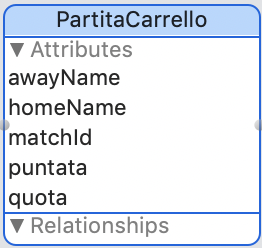
\includegraphics[width=0.2\textwidth]{images/DatiSchedina}
\end{figure}

\section{Client}
Per la realizzazione dell'applicazione si è optato per un back-end mobile, quindi un architettura solo client. Questa scelta deriva dal fatto che l'applicazione non ha la necessità di interfacciarsi con altri utenti e per i vari servizi fa uso di API terze. La comunicazione con i servizi terzi si basa su richieste HTTPS REST, in particolare tramite delle richieste GET.\\
Il client si basa sul tradizionale pattern MVC.
\begin{itemize}
	\item Model: in this package are contained all the classes about data shown to user, taken by the Controller and published by the View.
	\item View: in questo package sono contenuti tutti i componenti responsabili della visualizzazione dei dati e dell'interazione con l'utente
	\item Controller: in questo package sono contenuti tutti gli oggetti responsabili dell'interazione tra uno o più oggetti view dell'applicazione e uno o più oggetti model.
\end{itemize}

\chapter{Use case functional requirements analysis}
This section describes how actors can interact with iSport in order to use all the features implemented in the app. The focus of this part is on the front-end and we show the operations that can be performed by the actors without taking care of the system architecture behind the app.
\subsection*{Visualizzare Notizie}
\begin{tabular}{|c|p{0.8\textwidth}|}
	\hline
	\parbox[c][6ex]{6ex}{\centering \textbf{Name}} & Visualizzare Notizie\\
	\hline
	\parbox[c][6ex]{6ex}{\centering \textbf{Actor}} & User \\
	\hline
	\parbox[c][10ex]{15ex}{\centering \textbf{Entry Condition}} & L'attore ha scaricato l'applicazione\\
	\hline
	\parbox[c][6ex]{15ex}{\centering \textbf{Goal}} &  1, 2\\
	\hline
	\parbox[c][10ex]{12ex}{\centering \textbf{Event Flow}} & \begin{itemize}
		\item L'utente apre l'applicazione
		\item L'utente preme sulla tab "News"
		\item L'applicazione fornisce un elenco delle notizie principali
		\item L'utente preme sull'articolo di cui vuole visualizzare la notizia completa
		\item L'utente preme il tasto "Done" per terminare la lettura
	\end{itemize}\\
	\hline
	\parbox[c][7ex]{12ex}{\centering \textbf{Exit condition}} & L'utente ha letto la notizia di interesse. \\\hline
	\parbox[c][10ex]{13ex}{\centering \textbf{Exceptions}} & L'utente non è connesso alla rete e quindi non può inviare le richieste per ottenere gli articoli e quindi non può mostrarle. L'articolo è stato rimosso dal sito di origine, ma non nel database del servizio terzo \\ \hline	
\end{tabular}

\subsection*{Visualizzare Partite}
\begin{tabular}{|c|p{0.8\textwidth}|}
	\hline
	\parbox[c][6ex]{6ex}{\centering \textbf{Name}} & Visualizzare Partite\\
	\hline
	\parbox[c][6ex]{6ex}{\centering \textbf{Actor}} & User \\
	\hline
	\parbox[c][10ex]{15ex}{\centering \textbf{Entry Condition}} & L'attore ha scaricato l'applicazione\\
	\hline
	\parbox[c][6ex]{15ex}{\centering \textbf{Goal}} &  3\\
	\hline
	\parbox[c][10ex]{12ex}{\centering \textbf{Event Flow}} & \begin{itemize}
		\item L'utente apre l'applicazione
		\item L'utente preme sulla tab "Live"
		\item L'applicazione fornisce un elenco delle partite del giorno
	\end{itemize}\\
	\hline
	\parbox[c][7ex]{12ex}{\centering \textbf{Exit condition}} & L'utente ha visualizzato i risultati delle partite. \\\hline
	\parbox[c][10ex]{13ex}{\centering \textbf{Exceptions}} & L'utente non è connesso alla rete e quindi non può inviare le richieste per ottenere i risultati e quindi non può mostrargli. La connessione potrebbe essere debole e quindi non riuscire a ricevere i dati richiesti. \\ \hline	
\end{tabular}




\subsection*{Visualizzare Formazione Partita}
\begin{tabular}{|c|p{0.8\textwidth}|}
	\hline
	\parbox[c][6ex]{6ex}{\centering \textbf{Name}} & Visualizzare Formazione Partita\\
	\hline
	\parbox[c][6ex]{6ex}{\centering \textbf{Actor}} & User \\
	\hline
	\parbox[c][10ex]{15ex}{\centering \textbf{Entry Condition}} & L'attore ha scaricato l'applicazione\\
	\hline
	\parbox[c][6ex]{15ex}{\centering \textbf{Goal}} &  3, 6\\
	\hline
	\parbox[c][10ex]{12ex}{\centering \textbf{Event Flow}} & \begin{itemize}
		\item L'utente apre l'applicazione
		\item L'utente preme sulla tab "Live"
		\item L'applicazione fornisce un elenco delle partite del giorno
		\item L'utente preme sulla partita di cui vuole ottenere l'informazione richiesta
		\item L'utente preme sul bottone raffigurante il campo di gioco
	\end{itemize}\\
	\hline
	\parbox[c][7ex]{12ex}{\centering \textbf{Exit condition}} & L'utente ha visualizzato le formazioni delle due squadre della partita richiesta. \\\hline
	\parbox[c][10ex]{13ex}{\centering \textbf{Exceptions}} & L'utente non è connesso alla rete e quindi non può inviare le richieste per ottenere i risultati e quindi non può mostrargli. La connessione potrebbe essere debole e quindi non riuscire a ricevere i dati richiesti. \\ \hline	
\end{tabular}

\subsection*{Visualizzare Marcatori Partita}
\begin{tabular}{|c|p{0.8\textwidth}|}
	\hline
	\parbox[c][6ex]{6ex}{\centering \textbf{Name}} & Visualizzare Marcatori Partita\\
	\hline
	\parbox[c][6ex]{6ex}{\centering \textbf{Actor}} & User \\
	\hline
	\parbox[c][10ex]{15ex}{\centering \textbf{Entry Condition}} & L'attore ha scaricato l'applicazione\\
	\hline
	\parbox[c][6ex]{15ex}{\centering \textbf{Goal}} &  3, 4\\
	\hline
	\parbox[c][10ex]{12ex}{\centering \textbf{Event Flow}} & \begin{itemize}
		\item L'utente apre l'applicazione
		\item L'utente preme sulla tab "Live"
		\item L'applicazione fornisce un elenco delle partite del giorno
		\item L'utente preme sulla partita di cui vuole ottenere l'informazione richiesta
		\item L'utente preme sul bottone raffigurante un pallore
	\end{itemize}\\
	\hline
	\parbox[c][7ex]{12ex}{\centering \textbf{Exit condition}} & L'utente ha visualizzato i marcatori della partita richiesta. \\\hline
	\parbox[c][10ex]{13ex}{\centering \textbf{Exceptions}} & L'utente non è connesso alla rete e quindi non può inviare le richieste per ottenere i risultati e quindi non può mostrargli. La connessione potrebbe essere debole e quindi non riuscire a ricevere i dati richiesti. \\ \hline	
\end{tabular}
\subsection*{Visualizzare Statistiche Partita}
\begin{tabular}{|c|p{0.8\textwidth}|}
	\hline
	\parbox[c][6ex]{6ex}{\centering \textbf{Name}} & Visualizzare Statistiche Partita\\
	\hline
	\parbox[c][6ex]{6ex}{\centering \textbf{Actor}} & User \\
	\hline
	\parbox[c][10ex]{15ex}{\centering \textbf{Entry Condition}} & L'attore ha scaricato l'applicazione\\
	\hline
	\parbox[c][6ex]{15ex}{\centering \textbf{Goal}} &  3, 7\\
	\hline
	\parbox[c][10ex]{12ex}{\centering \textbf{Event Flow}} & \begin{itemize}
		\item L'utente apre l'applicazione
		\item L'utente preme sulla tab "Live"
		\item L'applicazione fornisce un elenco delle partite del giorno
		\item L'utente preme sulla partita di cui vuole ottenere l'informazione richiesta
		\item L'utente preme sul bottone raffigurante un grafico
	\end{itemize}\\
	\hline
	\parbox[c][7ex]{12ex}{\centering \textbf{Exit condition}} & L'utente ha visualizzato le statistiche della partita richiesta. \\\hline
	\parbox[c][10ex]{13ex}{\centering \textbf{Exceptions}} & L'utente non è connesso alla rete e quindi non può inviare le richieste per ottenere i risultati e quindi non può mostrargli. La connessione potrebbe essere debole e quindi non riuscire a ricevere i dati richiesti. \\ \hline	
\end{tabular}
\subsection*{Visualizzare Ammonizioni Partita}
\begin{tabular}{|c|p{0.8\textwidth}|}
	\hline
	\parbox[c][6ex]{6ex}{\centering \textbf{Name}} & Visualizzare Ammonizioni Partita\\
	\hline
	\parbox[c][6ex]{6ex}{\centering \textbf{Actor}} & User \\
	\hline
	\parbox[c][10ex]{15ex}{\centering \textbf{Entry Condition}} & L'attore ha scaricato l'applicazione\\
	\hline
	\parbox[c][6ex]{15ex}{\centering \textbf{Goal}} &  3, 5\\
	\hline
	\parbox[c][10ex]{12ex}{\centering \textbf{Event Flow}} & \begin{itemize}
		\item L'utente apre l'applicazione
		\item L'utente preme sulla tab "Live"
		\item L'applicazione fornisce un elenco delle partite del giorno
		\item L'utente preme sulla partita di cui vuole ottenere l'informazione richiesta
		\item L'utente preme sul bottone raffigurante un cartellino
	\end{itemize}\\
	\hline
	\parbox[c][7ex]{12ex}{\centering \textbf{Exit condition}} & L'utente ha visualizzato gli ammoniti ed espulsi della partita richiesta. \\\hline
	\parbox[c][10ex]{13ex}{\centering \textbf{Exceptions}} & L'utente non è connesso alla rete e quindi non può inviare le richieste per ottenere i risultati e quindi non può mostrargli. La connessione potrebbe essere debole e quindi non riuscire a ricevere i dati richiesti. \\ \hline	
\end{tabular}
\subsection*{Visualizzare Quote}
\begin{tabular}{|c|p{0.8\textwidth}|}
	\hline
	\parbox[c][6ex]{6ex}{\centering \textbf{Name}} & Visualizzare Quote\\
	\hline
	\parbox[c][6ex]{6ex}{\centering \textbf{Actor}} & User \\
	\hline
	\parbox[c][10ex]{15ex}{\centering \textbf{Entry Condition}} & L'attore ha scaricato l'applicazione\\
	\hline
	\parbox[c][6ex]{15ex}{\centering \textbf{Goal}} &  8\\
	\hline
	\parbox[c][10ex]{12ex}{\centering \textbf{Event Flow}} & \begin{itemize}
		\item L'utente apre l'applicazione
		\item L'utente preme sulla tab "Bet"
		\item L'applicazione fornisce un elenco delle quote dei principali pronostici delle partite odierne
	\end{itemize}\\
	\hline
	\parbox[c][7ex]{12ex}{\centering \textbf{Exit condition}} & L'utente ha visualizzatole quote delle partite odierne. \\\hline
	\parbox[c][10ex]{13ex}{\centering \textbf{Exceptions}} & L'utente non è connesso alla rete e quindi non può inviare le richieste per ottenere i risultati e quindi non può mostrargli. La connessione potrebbe essere debole e quindi non riuscire a ricevere i dati richiesti. \\ \hline	
\end{tabular}
\subsection*{Visualizzare la Schedina}
\begin{tabular}{|c|p{0.8\textwidth}|}
	\hline
	\parbox[c][6ex]{6ex}{\centering \textbf{Name}} & Aggiungere Partita a Schedina\\
	\hline
	\parbox[c][6ex]{6ex}{\centering \textbf{Actor}} & User \\
	\hline
	\parbox[c][10ex]{15ex}{\centering \textbf{Entry Condition}} & L'attore ha scaricato l'applicazione\\
	\hline
	\parbox[c][6ex]{15ex}{\centering \textbf{Goal}} &  9\\
	\hline
	\parbox[c][10ex]{12ex}{\centering \textbf{Event Flow}} & \begin{itemize}
		\item L'utente apre l'applicazione
		\item L'utente preme sulla tab "Bet"
		\item L'utente preme sul bottone raffigurante un carrello nella NavBar
	\end{itemize}\\
	\hline
	\parbox[c][7ex]{12ex}{\centering \textbf{Exit condition}} & L'utente visualizza i pronostici presenti nella schedina.\\\hline
	\parbox[c][10ex]{13ex}{\centering \textbf{Exceptions}} & L'utente non è connesso alla rete e quindi non può inviare le richieste per ottenere i risultati e quindi non può mostrargli. La connessione potrebbe essere debole e quindi non riuscire a ricevere i dati richiesti. \\ \hline	
\end{tabular}
\subsection*{Aggiungere Partita a Schedina}
\begin{tabular}{|c|p{0.8\textwidth}|}
	\hline
	\parbox[c][6ex]{6ex}{\centering \textbf{Name}} & Aggiungere Partita a Schedina\\
	\hline
	\parbox[c][6ex]{6ex}{\centering \textbf{Actor}} & User \\
	\hline
	\parbox[c][10ex]{15ex}{\centering \textbf{Entry Condition}} & L'attore ha scaricato l'applicazione\\
	\hline
	\parbox[c][6ex]{15ex}{\centering \textbf{Goal}} &  9\\
	\hline
	\parbox[c][10ex]{12ex}{\centering \textbf{Event Flow}} & \begin{itemize}
		\item L'utente apre l'applicazione
		\item L'utente preme sulla tab "Bet"
		\item L'applicazione fornisce un elenco delle quote dei principali pronostici delle partite odierne
		\item L'utente preme sulla quota relativa al pronostico e partita da aggiungere
	\end{itemize}\\
	\hline
	\parbox[c][7ex]{12ex}{\centering \textbf{Exit condition}} & L'utente ha aggiunto un pronostico di una partita alla schedina.\\\hline
	\parbox[c][10ex]{13ex}{\centering \textbf{Exceptions}} & L'utente non è connesso alla rete e quindi non può inviare le richieste per ottenere i risultati e quindi non può mostrargli. La connessione potrebbe essere debole e quindi non riuscire a ricevere i dati richiesti. \\ \hline	
\end{tabular}
\subsection*{Eliminare Partita da Schedina}
\begin{tabular}{|c|p{0.8\textwidth}|}
	\hline
	\parbox[c][6ex]{6ex}{\centering \textbf{Name}} & Eliminare Partita a Schedina\\
	\hline
	\parbox[c][6ex]{6ex}{\centering \textbf{Actor}} & User \\
	\hline
	\parbox[c][10ex]{15ex}{\centering \textbf{Entry Condition}} & L'attore ha scaricato l'applicazione\\
	\hline
	\parbox[c][6ex]{15ex}{\centering \textbf{Goal}} &  9\\
	\hline
	\parbox[c][10ex]{12ex}{\centering \textbf{Event Flow}} & \begin{itemize}
		\item L'utente apre l'applicazione
		\item L'utente preme sulla tab "Bet"
		\item L'utente preme sul bottone raffigurante un carrello nella NavBar
		\item L'utente effettua uno swipe verso sinistra sulla partita da eliminare
	\end{itemize}\\
	\hline
	\parbox[c][7ex]{12ex}{\centering \textbf{Exit condition}} & L'utente ha eliminato un pronostico di una partita alla schedina.\\\hline
	\parbox[c][10ex]{13ex}{\centering \textbf{Exceptions}} & Nessuna Eccezione\\ \hline	
\end{tabular}
\subsection*{Calcolare potenziale Vincita Schedina}
\begin{tabular}{|c|p{0.8\textwidth}|}
	\hline
	\parbox[c][6ex]{6ex}{\centering \textbf{Name}} & Calcolare potenziale Vincita Schedina\\
	\hline
	\parbox[c][6ex]{6ex}{\centering \textbf{Actor}} & User \\
	\hline
	\parbox[c][10ex]{15ex}{\centering \textbf{Entry Condition}} & L'attore ha scaricato l'applicazione\\
	\hline
	\parbox[c][6ex]{15ex}{\centering \textbf{Goal}} &  10\\
	\hline
	\parbox[c][10ex]{12ex}{\centering \textbf{Event Flow}} & \begin{itemize}
		\item L'utente apre l'applicazione
		\item L'utente preme sulla tab "Bet"
		\item L'utente preme sul bottone raffigurante un carrello nella NavBar
		\item L'utente inserisce l'importo da giocare nell'apposito input
		\item L'utente preme il tasto "Done"
	\end{itemize}\\
	\hline
	\parbox[c][7ex]{12ex}{\centering \textbf{Exit condition}} & L'utente visualizza la potenziale vincita della schedina attuale.\\\hline
	\parbox[c][10ex]{13ex}{\centering \textbf{Exceptions}} & Nessuna Eccezione \\ \hline	
\end{tabular}

\chapter{Sequence Diagram}
\chapter{User Interfaces}
\chapter{External Services and Libraries}

\chapter{Software System Attribute}
\section{Reliability}
\section{Availability}
\section{Security}
\section{Maintainability}
\section{Usability}

\chapter{Test Cases}
\chapter{Cost Estimation}







\end{document}
